\section{Experiments}

We trained adversarial nets on
a range of datasets including MNIST \cite{23_lecun1998gradient}, the Toronto Face Database (TFD) \cite{28_susskind2010toronto}, and CIFAR-10 \cite{21_krizhevsky2009learning}. The generator nets used a mixture of rectifier linear activations \cite{19_5459469,9_pmlr-v15-glorot11a} and sigmoid activations, while the discriminator net used maxout \cite{10_goodfellow2013maxoutnetworks} activations. Dropout \cite{17_hinton2012improvingneuralnetworkspreventing} was applied in training the discriminator net. While our theoretical framework permits the use of dropout and other noise at intermediate layer of the generator, we used noise as the input to only the bottommost layer of the generator network.

\begin{table}[ht]
	\centering
	\begin{tabular}{c|c|c}
		Model & MNIST & TFD\\
		\hline
		DBN \cite{3_pmlr-v28-bengio13} & $138 \pm 2$ & $1909 \pm 66$\\
		Stacked CAE \cite{3_pmlr-v28-bengio13} & $121 \pm 1.6$ & $\boldsymbol{2110 \pm 50}$\\
		Deep GSN \cite{6_pmlr-v32-bengio14} & $214 \pm 1.1$ & $1890 \pm 29$\\
		Adversarial nets & $\boldsymbol{225 \pm 2}$ & $\boldsymbol{2057\ \pm 26}$\\
	\end{tabular}
	\caption{Parzen window-based log-likelihood estimates. The reported numbers on MNIST are the mean log-likelihood of samples on test set, with the standard error of the mean computed across examples. On TFD, we computed the standard error across folds of the dataset, with a different $\sigma$ chosen using the validation set of each fold. On TFD, $\sigma$ was cross validated on each fold and mean log-likelihood on each fold were computed. For MNIST we compare against other models of the real-value (rather than binary) version of dataset.}
	\label{table: table 1}
\end{table}

We estimate probability of the test set data under $p_g$ by fitting a Gaussian Parzen window to the samples generated with $G$ and reporting the log-likelihood under thus distribution. The $\sigma$ parameter of the Gaussian was obtained by cross validation on the validation et. This procedure was introduced in Breuleux \emph{et al.} \cite{8_6796083} and used for various generative models for which the exact likelihood is not tractable \cite{25_10.5555/3042573.3042804,3_pmlr-v28-bengio13,5_bengio2014deepgenerativestochasticnetworks}. Results are reported in table \ref{table: table 1}
. This method of estimating the likelihood has somewhat high variance and does not perform well in high dimensional spaces but it is the best method available to our knowledge. Advances in generative models that can sample but not estimate likelihood directly motivate further research into how to evaluate such models.

In Figures %TODO: Figure 2 ref
and %TODO: Figure 3 ref
we show samples drawn from the generator net after training. While we make no claim that these samples are better than samples generated by existing methods, we believe that these samples are at least competitive with the better generative models in the literature and highlight the potential of the adversarial framework.

\begin{figure}[htb]
	\centering
	\subfigure[]{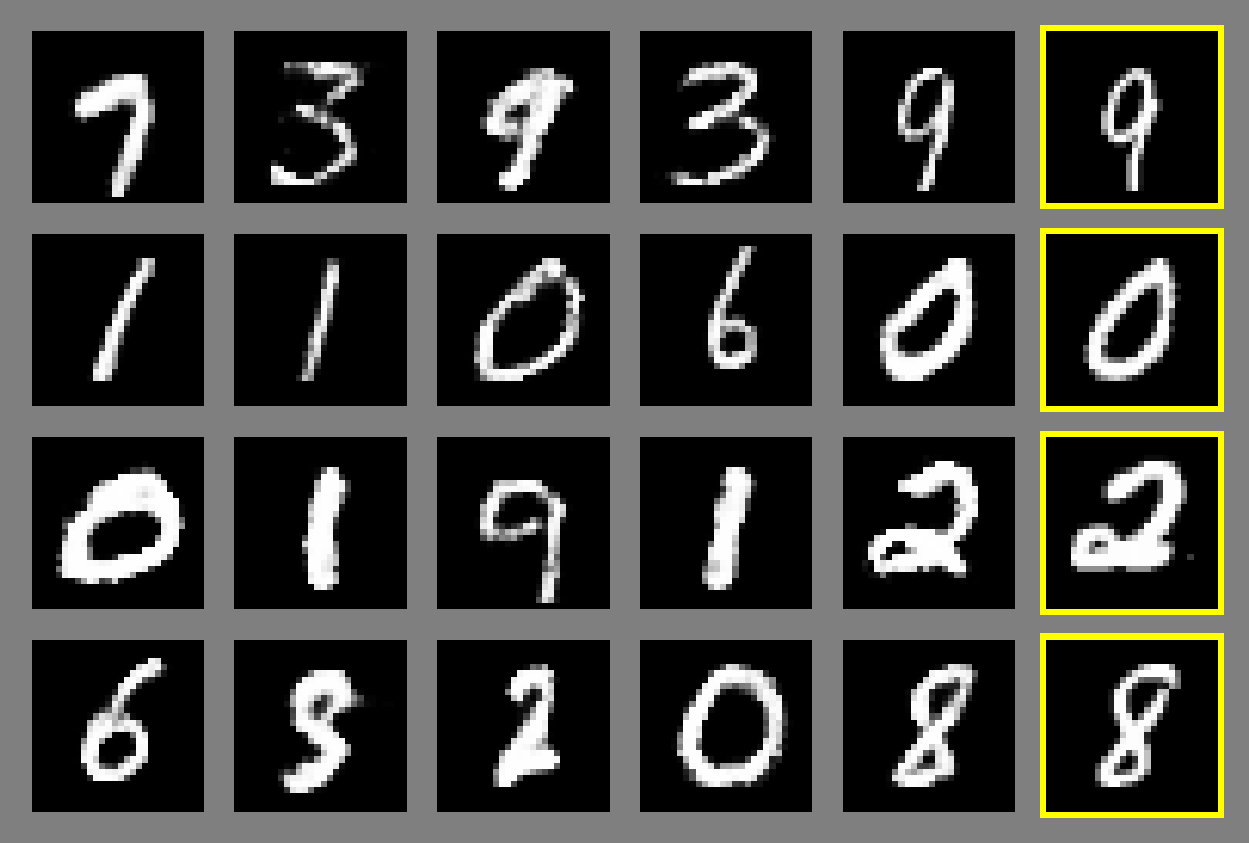
\includegraphics[width=0.45\textwidth]{figures/figure-2-sub-a.png}}
	\subfigure[]{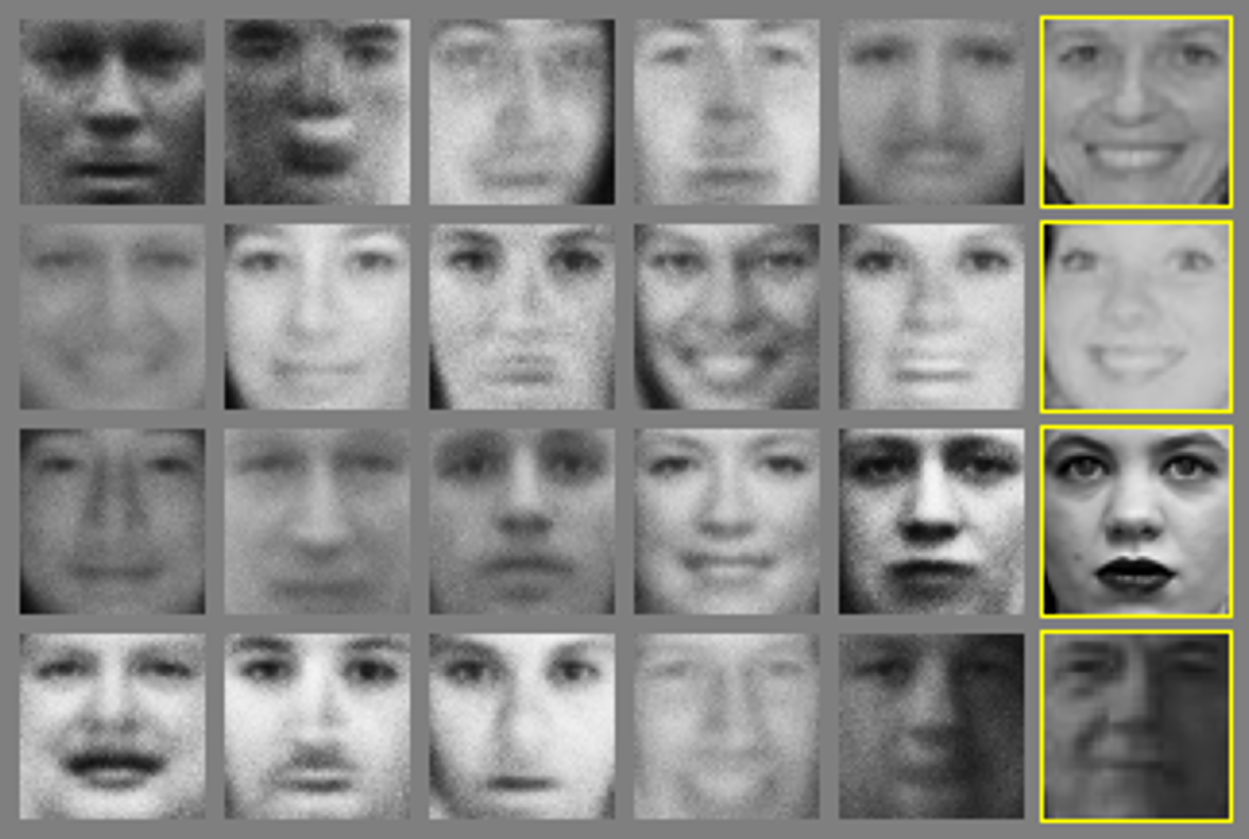
\includegraphics[width=0.45\textwidth]{figures/figure-2-sub-b.png}}
	\subfigure[]{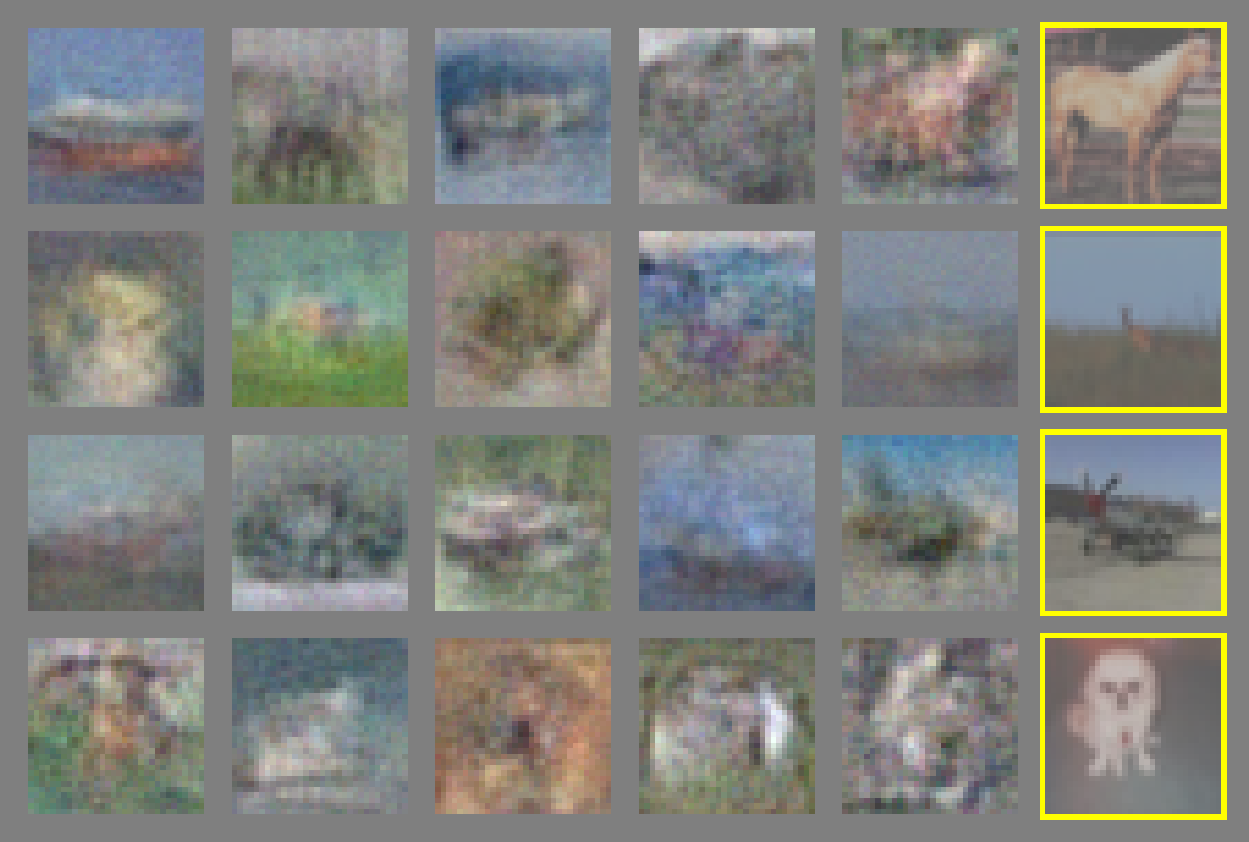
\includegraphics[width=0.45\textwidth]{figures/figure-2-sub-c.png}}
	\subfigure[]{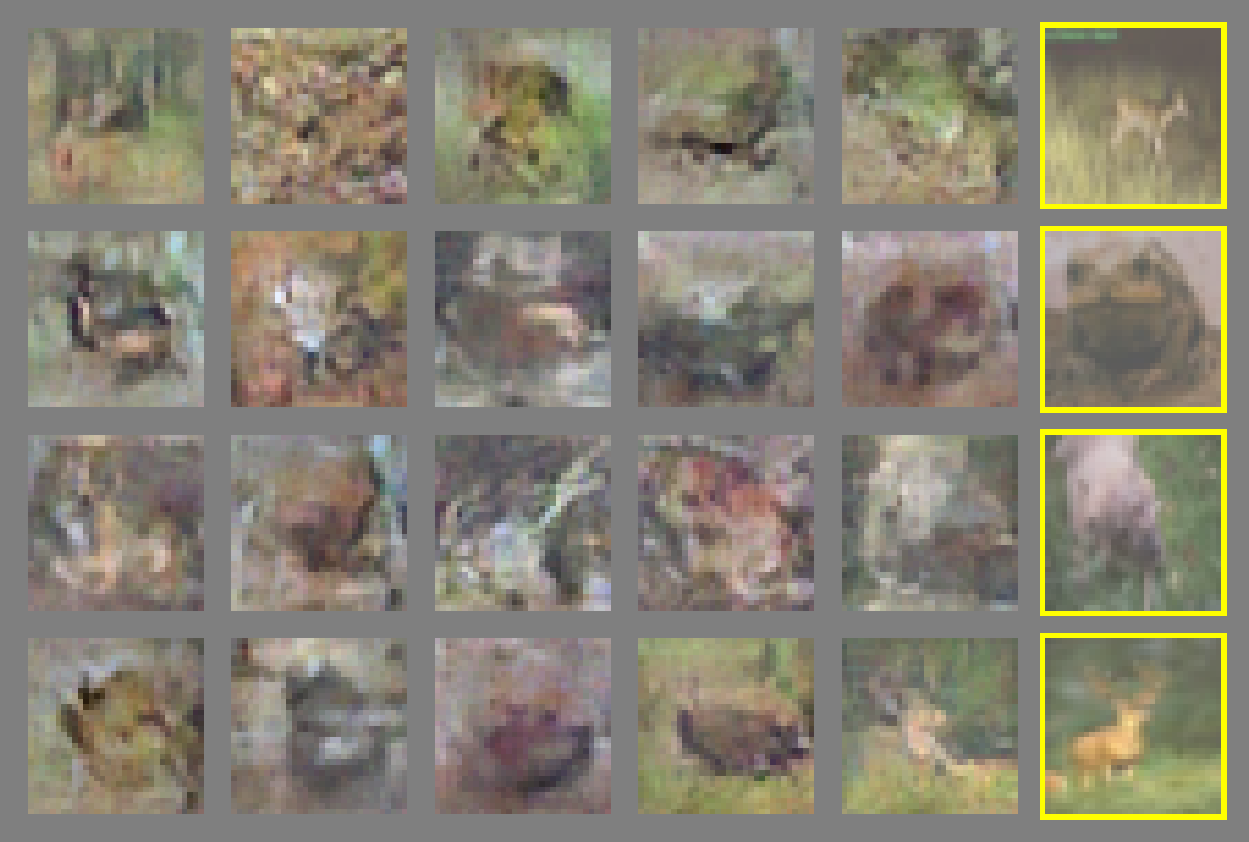
\includegraphics[width=0.45\textwidth]{figures/figure-2-sub-d.png}}
	\caption{Visualization of samples from the model. Rightmost column show the nearest training example of neighboring sample, in order to demonstrate that the model has not memorized the training set. Samples are fair random draws, no cherry-picked. Unlike most other Visualizations of deep generative models, these images show actual samples from the model distributions, not conditional means given samples of hidden units. Moreover, these samples are uncorrelated because the sampling process does not depend on Markov chain mixing. (a) MNIST (b) TFD (c) CIFAR-10 (fully connected model) (d) CIFAR-10 (convolutional discriminator and ''deconvolutional'' generator)}
\end{figure}

\begin{figure}[thb]
	\centering
	\resizebox{0.75\textwidth}{!}{
		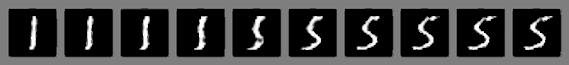
\includegraphics{figures/figure-3-left.pdf}
		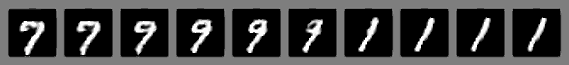
\includegraphics{figures/figure-3-right.pdf}
	}
	\caption{Digits obtained by linearly interpolating between coordinates in $\bz$ space of the full model.}
\end{figure}

\begin{table}
	\renewcommand\tabularxcolumn[1]{m{#1}}
	\begin{tabularx}{\textwidth}{>{\raggedright}c|X|X|X|X}%{c|l|l|l|l}
		& Deep directed graphical models & Deep undirected graphical models & Generative autoencoders & Adversarial models\\
		\hline
		Training & Inference needed during training. & Inference needed during training. MCMC needed to approximate partition function gradient. & Enforced tradeoff between mixing and power of reconstruction generation. & Synchronizing the discriminator with the generator. Helvetica\\
		\hline
		Inference & Learned approximate inference & Variational inference & MCMC-based inference & Learned approximate inference\\
		\hline
		Sampling & No difficulties & Requires Markov chain & Requires Markov chain & No difficulties\\
		\hline
		Evaluating $p(x)$ & Intractable, may be approximated with AIS & Intractable, may be approximated with AIS & Not explicitly represented, may be approximated with Parzen density estimation & Not explicitly represented, may be approximated with Parzen density estimation\\
		\hline
		Model design & Nearly all models incur extreme difficulty & Careful design needed to ensure multiple properties & Any differentiable function is theoretically permitted & Any differentiable function is theoretically permitted\\
	\end{tabularx}
	\caption{Challenges in generative modeling: a summary of the difficulties encountered by different approaches to deep generative modeling for each of the major operations involving a model.}
\end{table}